\let\negmedspace\undefined
\let\negthickspace\undefined
\documentclass[journal]{IEEEtran}
\usepackage[a5paper, margin=10mm, onecolumn]{geometry}
%\usepackage{lmodern} % Ensure lmodern is loaded for pdflatex
\usepackage{tfrupee} % Include tfrupee package

\setlength{\headheight}{1cm} % Set the height of the header box
\setlength{\headsep}{0mm}  % Set the distance between the header box and the top of the text

\usepackage{gvv}
\usepackage{cite}
\usepackage{amsmath,amssymb,amsfonts,amsthm}
\usepackage{algorithmic}
\usepackage{graphicx}
\usepackage{textcomp}
\usepackage{xcolor}
\usepackage{txfonts}
\usepackage{listings}
\usepackage{enumitem}
\usepackage{mathtools}
\usepackage{gensymb}
\usepackage{comment}
\usepackage{listings}
\def\inputGnumericTable{}                                 
\usepackage[latin1]{inputenc}                                 
\usepackage{color}                                            
\usepackage{array}                                            
\usepackage{longtable}                                       
\usepackage{calc}                                             
\usepackage{multirow}                                         
\usepackage{hhline}                                           
\usepackage{ifthen}                                           
\usepackage{lscape}

% Corrected equation environment commands
\newcommand{\BEQA}{\begin{eqnarray}}
\newcommand{\EEQA}{\end{eqnarray}}
\newcommand{\define}{\stackrel{\triangle}{=}}
\documentclass{article}
\usepackage{amsmath}
\usepackage{graphicx}
\usepackage{ifthen}
\usepackage{lscape}

\begin{document}

\bibliographystyle{IEEEtran}
\vspace{3cm}

\title{3-3.2-26}
\author{AI24BTECH11006 - Bugada Roopansha}
{\let\newpage\relax\maketitle}  % Prevents the new page after title

\renewcommand{\thefigure}{\theenumi}
\renewcommand{\thetable}{\theenumi}
\setlength{\intextsep}{10pt} % Space between text and floats
\textbf{Question}:\\
Construct a right triangle when one side is 3.5 cm, the sum of the other, and the hypotenuse is 5.5 cm.\\
\textbf{Solution}\\
\begin{table}[h!]
\centering
\begin{tabular}{|c|c|}
\hline
\textbf{Segment} & \textbf{Norm} \\ \hline
\( ||AB|| \) & $3.5$ \\ \hline
\( ||BC|| \) & Distance between B and C \\ \hline
\( ||AC|| \) & Distance between C and A \\ \hline
\end{tabular}
\caption{Norms of Segments \( ||AB||, ||BC||, \) and \( ||AC|| \)}
\end{table}

\[ 
||AB|| = 3.5 \, \text{cm}, \quad ||BC|| + ||AC|| = 5.5 \, \text{cm} \implies 
\]

\[ 
||AC|| = \sqrt{||AB||^2 + ||BC||^2} \implies 
\]

\[ 
5.5 - ||BC|| = \sqrt{(3.5)^2 + ||BC||^2} \implies 
\]

\[ 
(5.5 - ||BC||)^2 = (3.5)^2 + ||BC||^2 \implies 
\]

\[ 
30.25 - 11||BC|| + ||BC||^2 = 12.25 + ||BC||^2 \implies 
\]

\[ 
||BC|| = \frac{18}{11} \approx 1.64 \, \text{cm} \implies 
\]

\[ 
||AC|| = 5.5 - ||BC|| \approx 3.86 \, \text{cm} 
\]

\[ 
\mathbf{u} = \begin{bmatrix} 3.5 \\ 0 \end{bmatrix}, \quad \mathbf{c} = \begin{bmatrix} 3.5 \\ 1.64 \end{bmatrix} 
\]

\[ 
\mathbf{u} \cdot \mathbf{c} = 3.5 \cdot 3.5 = 12.25 
\]

\[ 
||\mathbf{u}|| = 3.5, \quad ||\mathbf{c}|| = \sqrt{(3.5)^2 + (1.64)^2} 
\]

\[ 
\cos(\theta) = \frac{12.25}{3.5 \cdot \sqrt{3.5^2 + 1.64^2}} 
\]

\[ 
\theta = \arccos\left(\cos(\theta)\right) \approx 34.89^\circ 
\]

\begin{figure}[h!]
\centering
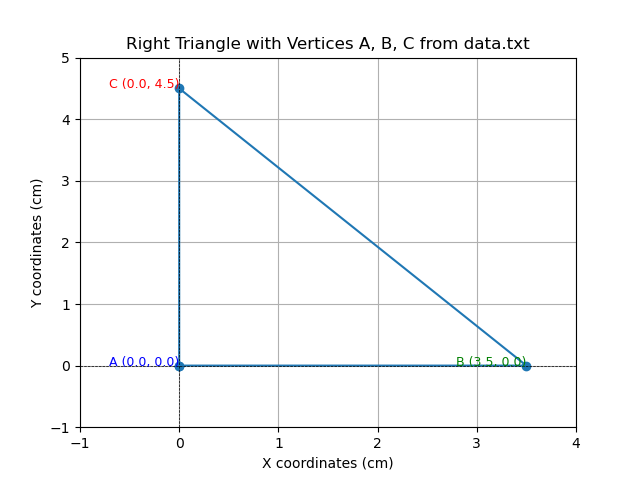
\includegraphics[width=1\textwidth]{fig.png} % Replace with your image file
\caption{Right triangle with one side of 3.5 cm and the sum of the other side and hypotenuse equal to 5.5 cm.}
\end{figure}

\end{document}

